\section{Data description and Visualisation}

The dataset chosen for this assignment is the meteorite compositional data. The data consists of 12 samples 
from different geographical locations see Fig. \ref{fig:locations}, each sample is composition consisting of 9 parts. The 9 parts are the metaloxides: \{FeO, Al2O3, MgO, SiO2, MnO\}, the metals \{Fw, Ni, Co\} and Carbon(C). Besides a location, each sample also had chondrite type, a summary of these can be seen in tabble \ref{tab:chondrite-types}.

\begin{table}[H]
\centering
\begin{tabular}{@{}ll@{}}
\toprule
\textbf{Code} & \textbf{Meaning} \\ \midrule
cc & \textbf{Carbonaceous chondrite}: rich in carbon, hydrated minerals, primitive, volatile-rich. \\
hc & \textbf{High-iron chondrite} (H chondrite): ordinary chondrite with high metal content. \\
lc & \textbf{Low-iron chondrite} (L chondrite): ordinary chondrite with lower metal content. \\ \bottomrule
\end{tabular}
\caption{Summary of meteorite chondrite types and their meanings.}
\label{tab:chondrite-types}
\end{table}



%Notes 
%Something abouth the fact that data is not closed to same amount
%Be clear about the fact that the data is closed for the remainder of the assignment
%Something about waht makes the data compositional 
% ALso just say something abouth the fact that there is generally a lot more of MgO SiO2 and FeO than any of the aprts:w




\begin{figure}[htbp]
    \centering
    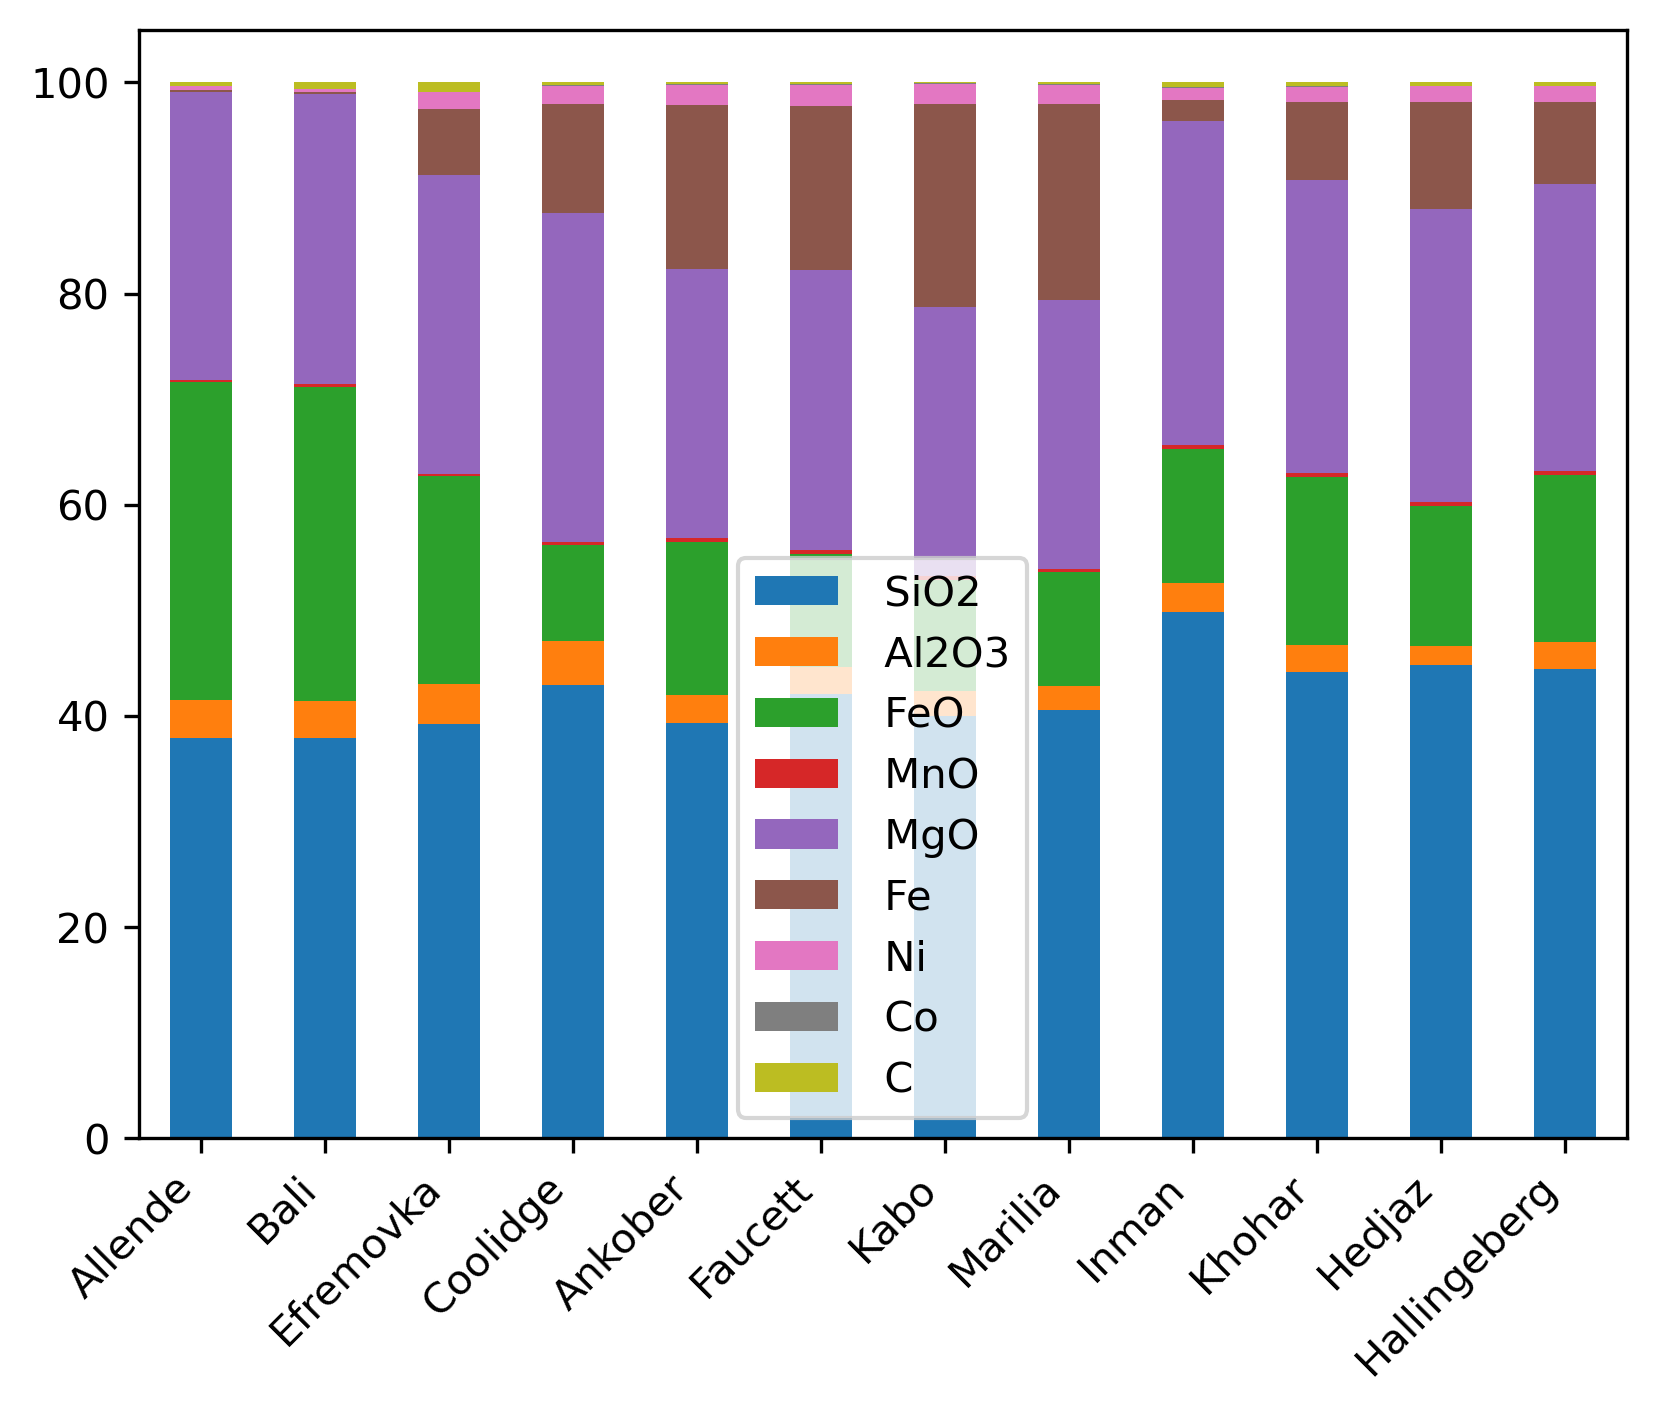
\includegraphics[width=0.8\textwidth]{figures/stacked_bar.png}
    \caption{Example plot showing the chemical composition of meteorites.}
    \label{fig:stacked}
\end{figure}






\begin{figure}[H]
    \centering
    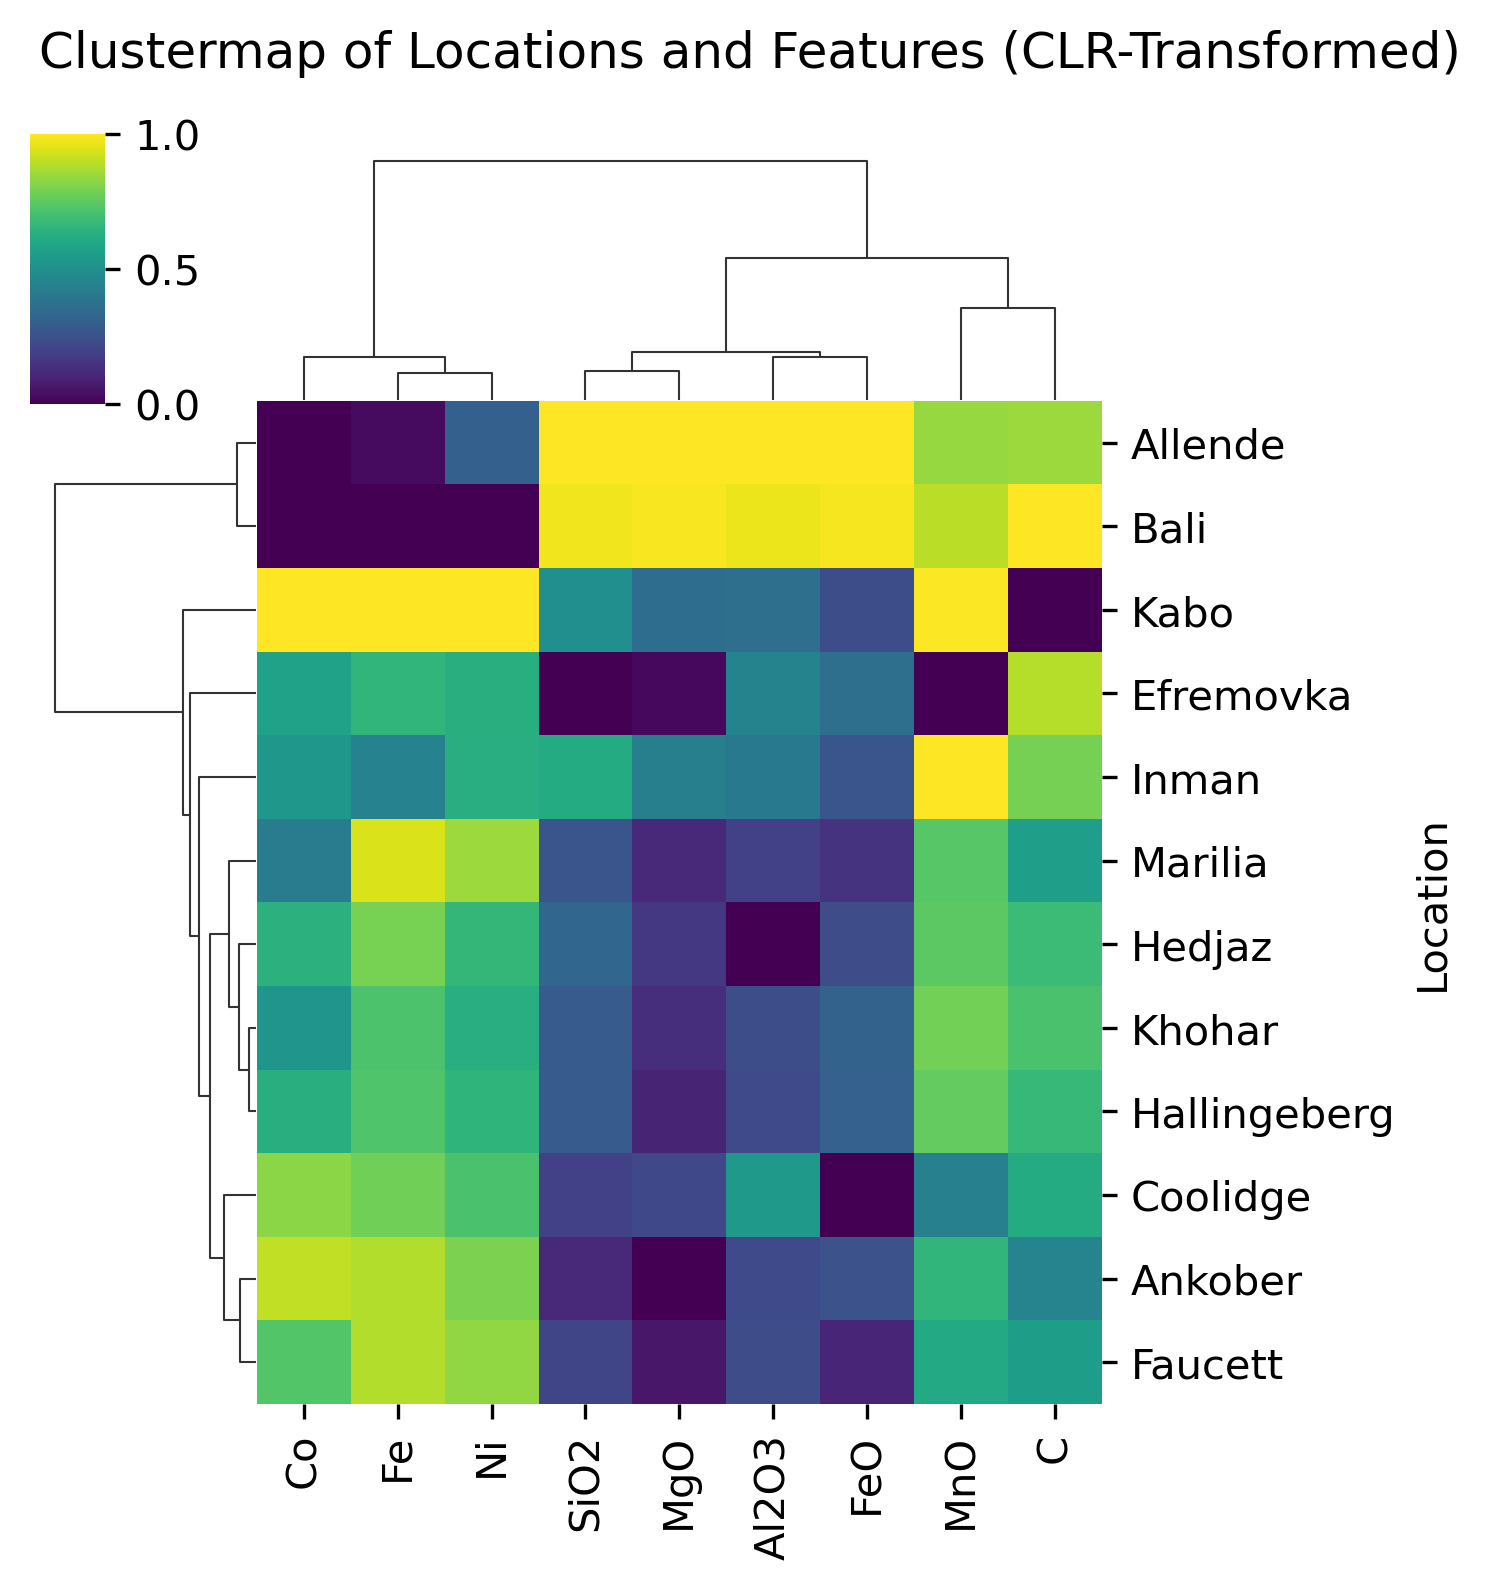
\includegraphics[width=0.4\textwidth]{figures/clustermap.png}
    \caption{Example plot showing the chemical composition of meteorites.}
    \label{fig:clustermap}
\end{figure}



